This chapter describes how to simulate contamination incidents in a water distribution network, 
which is one of the first steps before designing a water quality sensor network or evaluating
response actions to a contamination incident. The \code{tevasim} subcommand simulates 
the hydraulics and contaminant transport within a water distribution network model, which 
consists of pipe, node, pump, valve, storage tank and reservoir components. 
The \code{tevasim} subcommand uses the hydraulic engine from EPANET 2.00.12 to solve the flow 
continuity and headloss equations \citep{EPANETusermanual}. Water quality simulations are calculated
using either EPANET 2.00.12 \citep{EPANETusermanual}, EPANET-MSX \citep{ShaUbeRos11}
or Merlion \citep{Merlion12}. To increase efficiency when simulating a large ensemble 
of contamination incidents, the \code{tevasim} subcommand uses a single hydraulic simulation 
to simulate an ensemble of water quality simulations. 
A flowchart representation of the \code{tevasim} subcommand is shown in Figure \ref{fig:tevasim-flowchart}. 
The utility network model is defined by an EPANET compatible network model (INP format) in WST. 
The simulation input is supplied through the \code{tevasim} WST configuration file.

\begin{figure}[h]
  \centering
  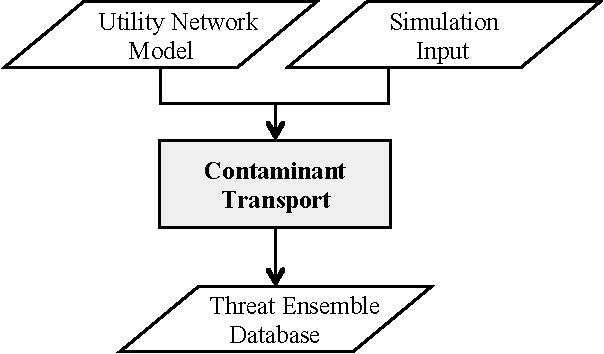
\includegraphics[scale=0.80]{graphics/tevasim_flowchart.pdf}
  \caption{Contaminant transport simulation flowchart.}
  \label{fig:tevasim-flowchart}
\end{figure}

\section{Hydraulic and Water Quality Analysis}
Three water quality simulators, EPANET, EPANET-MSX and Merlion, can be used within WST. These 
simulators are explained in more detail in the following subsections.
\subsection{EPANET and EPANET-MSX}\label{epanet}
EPANET performs extended-period simulation of the hydraulic and water quality 
behavior within pressurized pipe networks. These models can evaluate the 
expected flow in water distribution systems, and model the transport of 
contaminants and related chemical interactions. The multi-species extension, 
EPANET-MSX, is also included in WST to simulate contamination incidents 
using multi-species reactions. Any reaction dynamics between chemical and/or 
biological species (e.g., chemical-chemical, chemical-biological or
biological-biological) can be modeled and simulated using EPANET-MSX. 
EPANET-MSX can be used in sensor network design (\code{sp} subcommand) and 
booster station placement (\code{booster\_msx} subcommand). More specifics 
on these applications can be found in Chapters \ref{chap:sp} and \ref{chap:booster}. 
Additional information on EPANET can be found at 
\url{https://www.epa.gov/water-research/epanet}
and in the EPANET 2.00.12 user manual \citep{EPANETusermanual}. Additional information 
on EPANET-MSX can be found in the EPANET-MSX user manual \citep{ShaUbeRos11}.

\subsection{Merlion}\label{merlion}
The \code{tevasim} subcommand also includes a water quality modeling framework
called Merlion. Unlike EPANET, Merlion does not model bulk or wall
reactions. Given hydraulic information from simulation packages like
EPANET or experimental data, Merlion models the transport of a substance
as it spreads through the water distribution system based on the network
dynamic flow patterns. Merlion first formulates a linear water quality model 
with explicit all-to-all mapping (inputs include injections at all possible nodes 
and time steps, and outputs include concentrations at all possible nodes and 
time steps). This model is then used for forward
tracing simulations by first specifying the injection profile and
then solving the system for the network concentration profile. The linear model 
can also be embedded within other numerical
applications or for analysis in many security applications. Using Merlion in the   
\code{tevasim} subcommand can be faster for multi-scenario simulations; however,
it is also more memory intensive. Merlion can also be used to  
identify booster station locations, contaminant source injection locations 
and manual grab sample locations. More specifics about these applications are in Chapters 
\ref{chap:booster}, \ref{chap:inversion} and \ref{chap:grabsample}. 
More information on Merlion can be found in Section \ref{appendixMerlion} and \citet{Merlion12}.

\section{Contaminant Transport Scenarios}\label{sec:scenarios}
Contaminant transport scenarios can be defined directly in a WST configuration file
or by using a TSI or TSG file. These options are set in the scenario
block of the configuration file for all of the WST subcommands that require scenarios.

The recommended approach is to define the contamination transport scenarios directly in 
the scenario block of the WST configuration file. The options that must be set are 
the location, type, strength, species (required only for EPANET-MSX) 
and start and end times for the contamination scenarios. 
The injection location can be specified by a list of EPANET node IDs, 
or by the key words NZD (non-zero demand nodes) or ALL (all nodes) to create an ensemble of contaminant scenarios. 
The injection type can be CONCEN, MASS, FLOWPACED or SETPOINT as defined in the EPANET user manual\citep{EPANETusermanual}.  
CONCEN represents the concentration of an external source entering a node and 
applies only when the node has a net negative demand (i.e., flows into the network). 
MASS, FLOWPACED and SETPOINT represent booster sources, 
where a contaminant is injected directly into the network regardless of nodal demand.
A MASS source type adds a fixed mass flow to that resulting from inflow to the node, while 
a FLOWPACED booster adds a fixed concentration to the resultant inflow concentration at the node.
A SETPOINT booster fixes the concentration leaving the node as long as the 
inflow concentration was below the setpoint.
The strength of a MASS source is in units of mass flow per minute, while
CONCEN, FLOWPACED and SETPOINT sources are in units of concentration (mass per volume). 
The configuration file defines injection time in minutes and strength in mg/L or mg/min 
depending on the injection type.

Alternatively, the contamination transport scenarios can be defined using a TSI or TSG file. 
Each line of a TSI file specifies a single contaminant scenario by listing the 
injection location, type, species (required only for EPANET-MSX), strength and time frame. Each scenario can include 
multiple injection locations and multiple injection species with unique injection strengths and
time frames. This format allows for the greatest flexibility in combined scenario options.  
For more detail on the TSI file, see File Formats Section \ref{formats_tsiFile}.

The TSG file is a short hand format of the more detailed TSI file. 
Multiple injection locations can be specified on a single line. All permutations of the 
combined locations are used to create multiple scenarios. Each line of the TSG file is limited 
to a single injection species and time frame. For more detail on the TSG file, see File Formats Section \ref{formats_tsgFile}.
The TSI and TSG files specify the injection time frame in seconds (which is different than 
the units specified for the start and end times in the configuration file) and 
the strength units depend on the INP network model file units. 

Specifying a TSI file overrides the TSG file, as well as the location, 
type, strength, species, start time and end time options specified in the WST configuration file.  
Specifying a TSG file overrides the location, type, strength, species, start time and 
end time options specified in the WST configuration file.   

\section{\code{tevasim} Subcommand}

The \code{tevasim} subcommand is executed using the following command line:
\begin{unknownListing}
wst tevasim <configfile> 
\end{unknownListing}
where \code{configfile} is a WST configuration file in the YAML format.  

The \code{---help} option prints information about this subcommand, such as usage,
arguments and a brief description:

\begin{unknownListing}
wst tevasim --help
\end{unknownListing}

\subsection{Configuration File}

The \code{tevasim} subcommand generates a template configuration file using the following command line:

\begin{unknownListing}
wst tevasim --template <configfile>
\end{unknownListing}

The \code{tevasim} WST template configuration file is shown in Figure \ref{fig:tevasim_template}. Brief descriptions 
of the options are included in the template after the \# sign.  

\begin{figure}[h]
  \unknownInputListing{examples/tevasim_config.yml}{}{1}{21}
  \caption{The \code{tevasim} configuration template file.}
  \label{fig:tevasim_template}
\end{figure}
  
\subsection{Configuration Options}

Full descriptions of the WST configuration options used by the \code{tevasim} subcommand are listed below.
\begin{description}[topsep=0pt,parsep=0.5em,itemsep=-0.4em]
  \item[{network}]\hfill
  \begin{description}[topsep=0pt,parsep=0.5em,itemsep=-0.4em]
    \item[{epanet file}]\hfill
\\ The name of the EPANET 2.00.12 input (INP) file that defines the water distribution
                network model.
                
                Required input.
  \end{description}
  \item[{scenario}]\hfill
  \begin{description}[topsep=0pt,parsep=0.5em,itemsep=-0.4em]
    \item[{location}]\hfill
\\A list that describes the injection locations for the contamination scenarios.
                The options are: (1) ALL, which denotes all nodes (excluding tanks and reservoirs)
                as contamination injection locations; (2) NZD, which denotes all nodes with
                non-zero demands as contamination injection locations; or (3) an EPANET node ID, 
                which identifies a node as the contamination injection location. This allows 
                for an easy specification of single or multiple contamination scenarios.
                
                Required input unless a TSG or TSI file is specified.
    \item[{type}]\hfill
\\The injection type for the contamination scenarios. The options are MASS, CONCEN, FLOWPACED or SETPOINT. 
                See the EPANET 2.00.12 user manual for additional information about source types \citep{EPANETusermanual}.
                
                Required input unless a TSG or TSI file is specified.
    \item[{strength}]\hfill
\\The amount of contaminant injected into the network for the contamination scenarios.  
                If the type option is MASS, then the units for the strength are in mg/min. 
                If the type option is CONCEN, FLOWPACED or SETPOINT, then units are in mg/L.
                
                Required input unless a TSG or TSI file is specified.
    \item[{species}]\hfill
\\The name of the contaminant species injected into the network. This is the name of a single species. 
                It is required when using EPANET-MSX, since multiple species might be simulated, but
                only one is injected into the network. For cases where multiple contaminants are injected,
                a TSI file must be used.
                
                Required input for EPANET-MSX unless a TSG or TSI file is specified.
    \item[{start time}]\hfill
\\The injection start time that defines when the contaminant injection begins. 
                The time is given in minutes and is measured from the start of the simulation. 
                For example, a value of 60 represents an injection that starts at hour 1 of the simulation.
                
                Required input unless a TSG or TSI file is specified.
    \item[{end time}]\hfill
\\The injection end time that defines when the contaminant injection stops.				
                The time is given in minutes and is measured from the start of the simulation.
                For example, a value of 120 represents an injection that ends at hour 2 of the simulation.
                
                Required input unless a TSG or TSI file is specified.
    \item[{tsg file}]\hfill
\\The name of the TSG scenario file that defines the ensemble of contamination
                scenarios to be simulated. Specifying a TSG file will
                override the location, type, strength, species and start and end times options specified in
                the WST configuration file. The TSG file format is documented in File Formats Section \ref{formats_tsgFile}.
                
                Optional input.
    \item[{tsi file}]\hfill
\\The name of the TSI scenario file that defines the ensemble of contamination
                scenarios to be simulated. Specifying a TSI file will
                override the TSG file, as well as the location, type, strength, species and start and end time options specified in
                the WST configuration file. The TSI file format is documented in File Formats Section \ref{formats_tsiFile}.
                
                Optional input.
    \item[{signals}]\hfill
\\Name of file or directory with information to generate 
                or load signals. If a file is provided the list of INP-TSG tuples
                 will be simulated and the information stored in signals files. If
                a directory with the signals files is specified, the signal files will
                be read and loaded in memory. This input is only valid for the uq
                subcommand and the grabsample subcommand with probability based formulations.

                Optional input.
    \item[{msx file}]\hfill
\\The name of the EPANET-MSX multi-species file that defines the multi-species reactions to
                be simulated using EPANET-MSX.
                
                Required input for EPANET-MSX.
    \item[{msx species}]\hfill
\\The name of the MSX species whose concentration profile will be saved by the EPANET-MSX simulation
                and used for later calculations.
                
                Required input for EPANET-MSX.
    \item[{merlion}]\hfill
\\A flag to indicate if the Merlion water quality
                simulator should be used. The options are true or false. 
                If an MSX file is provided, EPANET-MSX will be used.
                
                Required input, default = false.
  \end{description}
  \item[{configure}]\hfill
  \begin{description}[topsep=0pt,parsep=0.5em,itemsep=-0.4em]
    \item[{output prefix}]\hfill
\\The prefix used for all output files.
                
                Required input.
    \item[{output directory}]\hfill
      \\The output directory to store the results.
    \item[{debug}]\hfill
\\The debugging level (0 or 1) that indicates the amount of debugging 
                information printed to the screen, log file and output yml file. 
                
                Optional input, default = 0 (lowest level).
  \end{description}
\end{description}


\subsection{Subcommand Output}

The \code{tevasim} subcommand creates 
two output files, one is in the YAML file format and the other is a log file.
The YAML file is called <output prefix>tevasim\_output.yml  
and the log file is <output prefix>tevasim\_output.log. The YAML file 
contains the name of the EPANET report file, the name of the binary ERD database file, 
the run date and the CPU time. 
The EPANET report file and binary ERD database files are described below.
The log file contains basic debugging information.

\begin{itemize}
\item EPANET report: This file provides information on the EPANET simulations. 
The EPANET report file format is described in Appendix C.3 of the EPANET 2.00.12 Users Manual \citep{EPANETusermanual}.
\item ERD database: The database contains the simulation results, 
and is stored in four files: header file, index file, hydraulics file and a water 
quality file. The ERD database format is described in \citet{ERDusermanual}. This files is not
intended to be read by users but rather is read by other WST subcommands.
\end{itemize}

\section{Contaminant Transport Examples}\label{tevasim_example}

An EPANET network model (INP format) and a configuration file are required to 
run the \code{tevasim} subcommand.  

The \code{tevasim} template configuration file uses the EPANET Example Network 3 (Net3.inp).  
The network is shown in Figure \ref{fig:Net3}. 
Net3 contains 92 junctions, 2 reservoirs and 3 tanks. This network has 59 non-zero 
demand (NZD) nodes. The network file is setup to run a 
48-hour hydraulic and water quality simulation. A 1-hour 
hydraulic time step and 5-minute water quality time step are used.

\begin{figure}[h]
  \centering
  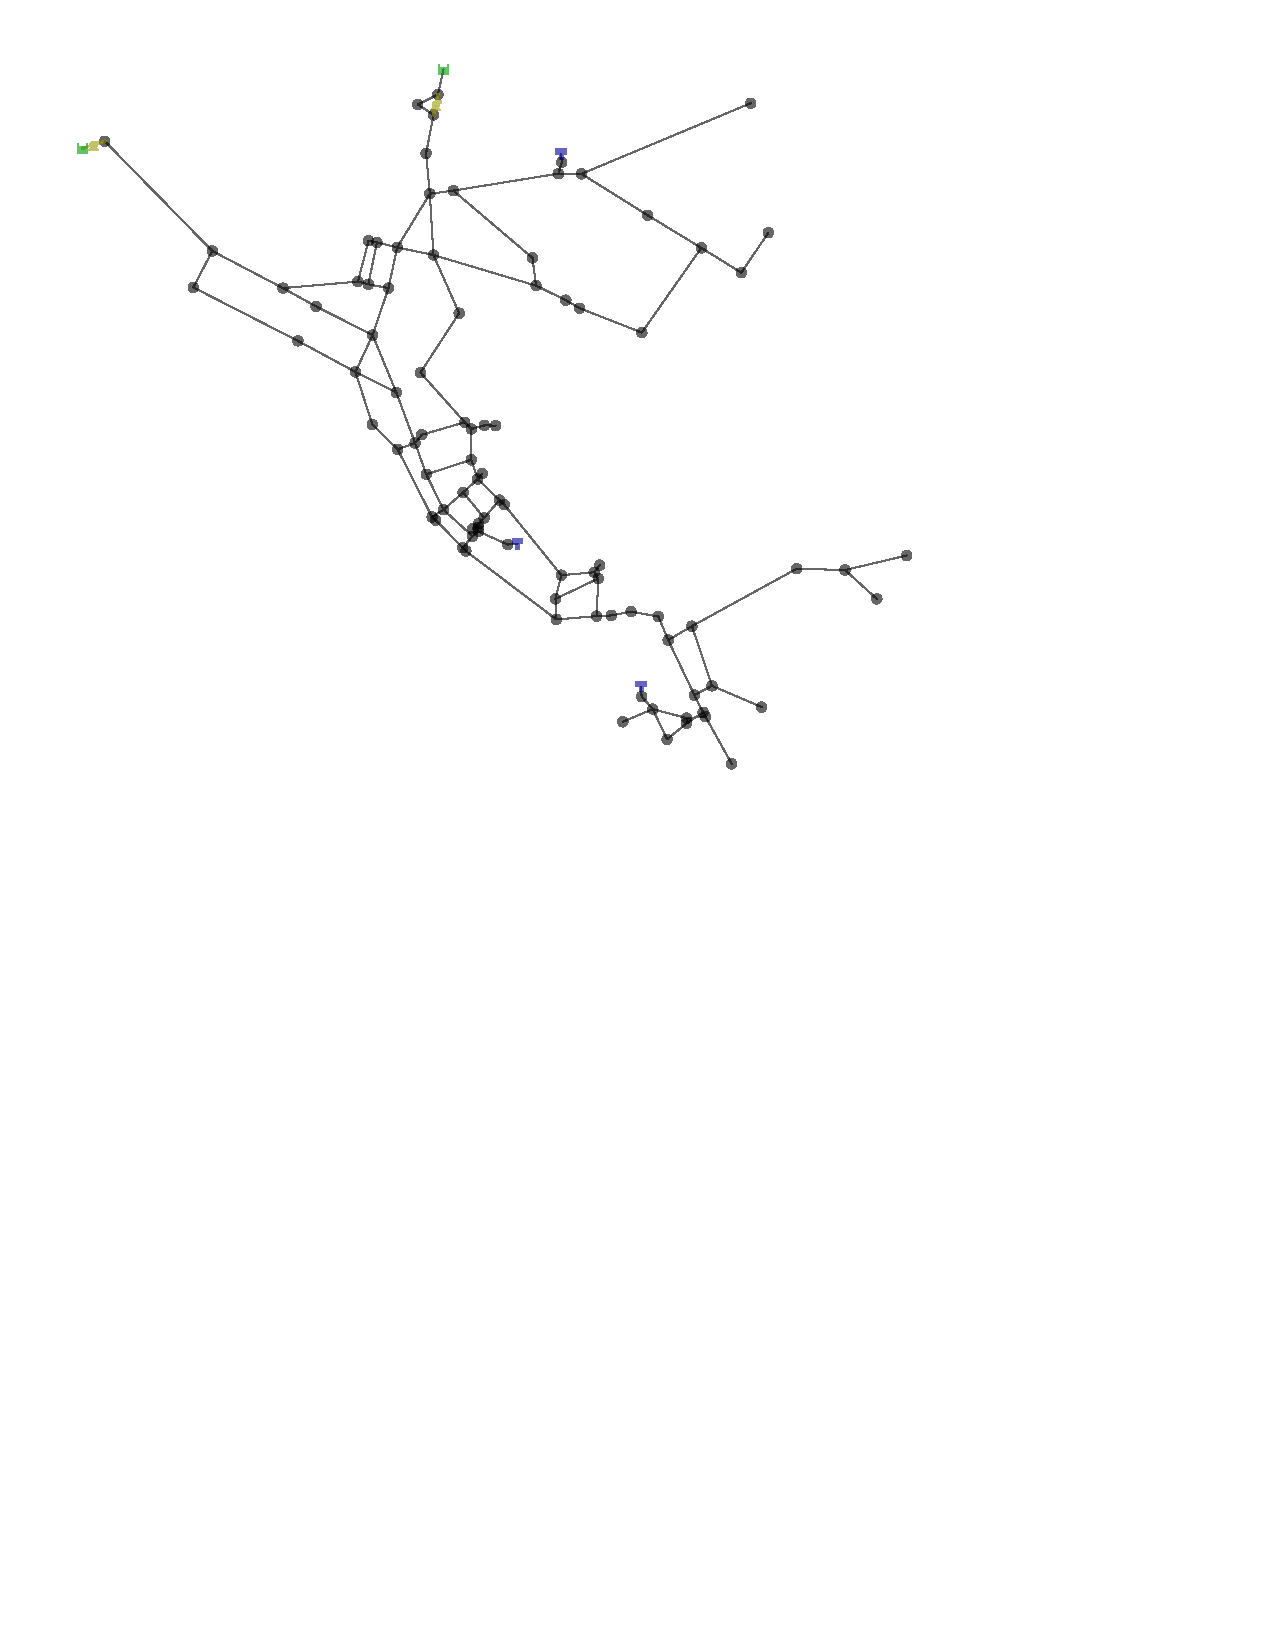
\includegraphics[scale=0.80]{graphics/Net3.pdf}
  \caption{Layout of the EPANET Example Network 3.}
  \label{fig:Net3}
\end{figure}

The scenario ensemble in the \code{tevasim} template configuration file defines 
a contaminant injection from each NZD node, with a MASS injection of 100 mg/L, starting 
at time 0 and injecting for 24 hours (1440 minutes).  

To define scenarios that start and stop at multiple times, a TSG file can be 
used to define the scenario set. Figure \ref{fig:Net3tsg} shows the example TSG file, Net3.tsg, in which the 
contamination scenarios are injected at all NZD nodes 
starting at 12 am, 6 am, 12 pm and 6 pm for a total of 236 scenarios. Each injection 
lasts 24 hours and injects a contaminant at 100 mg/L.

\begin{figure}[h!]
  \unknownInputListing{../../examples/Net3/Net3.tsg}{}{1}{8}
  \caption{Example TSG contamination scenario file.}
  \label{fig:Net3tsg}
\end{figure}

\subsection{Example 1}

The first example uses the Net3.inp network file, the contamination scenario set defined by Net3.tsg 
and the Merlion water quality model. The configuration file, tevasim\_ex1.yml, for this example is shown in Figure \ref{fig:tevasim_ex1}.  

\begin{figure}[h!]
  \unknownInputListing{../../examples/tevasim_ex1.yml}{}{1}{8}
  \caption{The \code{tevasim} configuration file for example 1.}
  \label{fig:tevasim_ex1}
\end{figure}

The example can be executed using the following command line:

\begin{unknownListing}
wst tevasim tevasim_ex1.yml
\end{unknownListing}

\FloatBarrier 
\subsection{Example 2}

The second example uses EPANET-MSX to simulate the transport of multiple contaminants. 
For a multi-species simulation, a MSX file and the MSX species must be added to the 
\code{tevasim} configuration file. The MSX species is the species whose concentration profile
will be saved by EPANET-MSX to be used for future calculations. The MSX species can be different
than the species which is injected into the network. The configuration file, tevasim\_ex2.yml, 
for this example is shown in Figure \ref{fig:tevasim_ex2}. The example uses the Net3.inp network file 
and the MSX file, Net3\_EColi\_TSB.msx, which simulates the reaction dynamics between
$Escherichia~coli$, chlorine and a tryptic soy broth (TSB), a nutrient broth that helps to grow bacteria. 
For more information about this specific reaction dynamics, see the $E.~coli$-TSB model 
described in \citet{MurrayAdcockRiceUberHatchett11}. In this example, both the species and MSX species are the
same.

\begin{figure}[h]
  \unknownInputListing{../../examples/tevasim_ex2.yml}{}{1}{17}
  \caption{The \code{tevasim} configuration file for example 2.}
  \label{fig:tevasim_ex2}
\end{figure}

The example can be executed using the following command line:

\begin{unknownListing}
wst tevasim tevasim_ex2.yml
\end{unknownListing}

To simulate the simultaneous injection of two species, a TSI file is needed. For example, the TSI file, 
Net3\_EColi\_TSB.tsi, defines the simultaneous injection of $E.~coli$ and TSB at multiple locations 
within Net 3. The TSI file contains explicit injections for the 59 NZD nodes used in example 1, with 
four species injected per node.
